\subsection{Overview}

\begin{figure}[H]
    \centering
    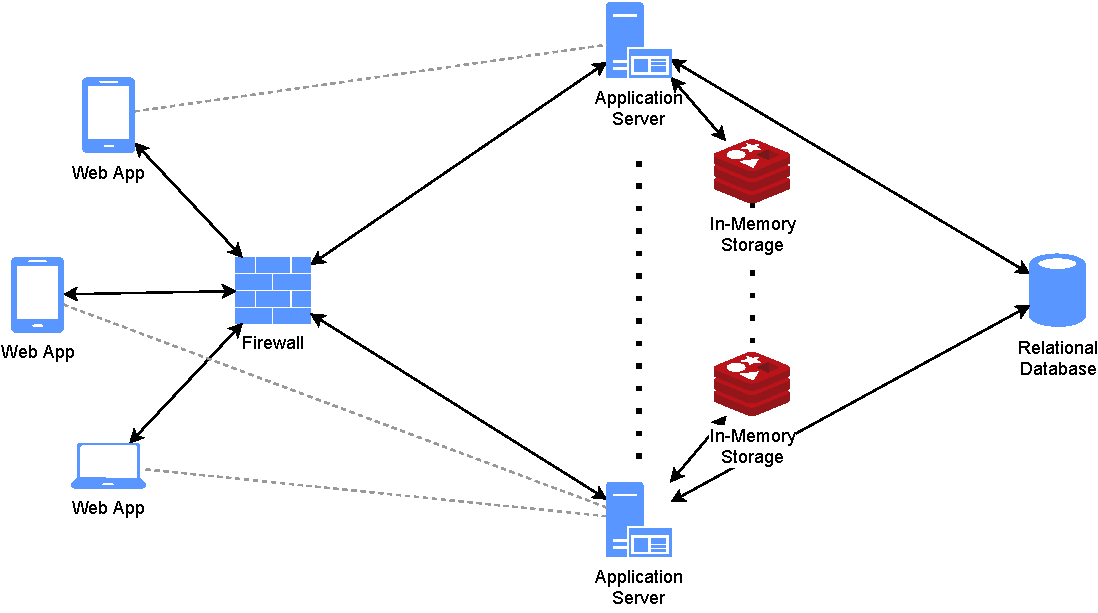
\includegraphics[width=.85\textwidth]{Images/overview.pdf}
    \caption{\label{fig:world_machine} Architecture overview}
\end{figure}
The figure above shows an high level representation of the \emph{CLup} system architecture.
Two parts can be easily distinguished, separated by the firewall: the Client Web Application and the Application Server with its data storage.
Further details on the System components and their interactions will be examined in the following sections.

\subsection{Component view}

\begin{figure}[H]
    \centering
    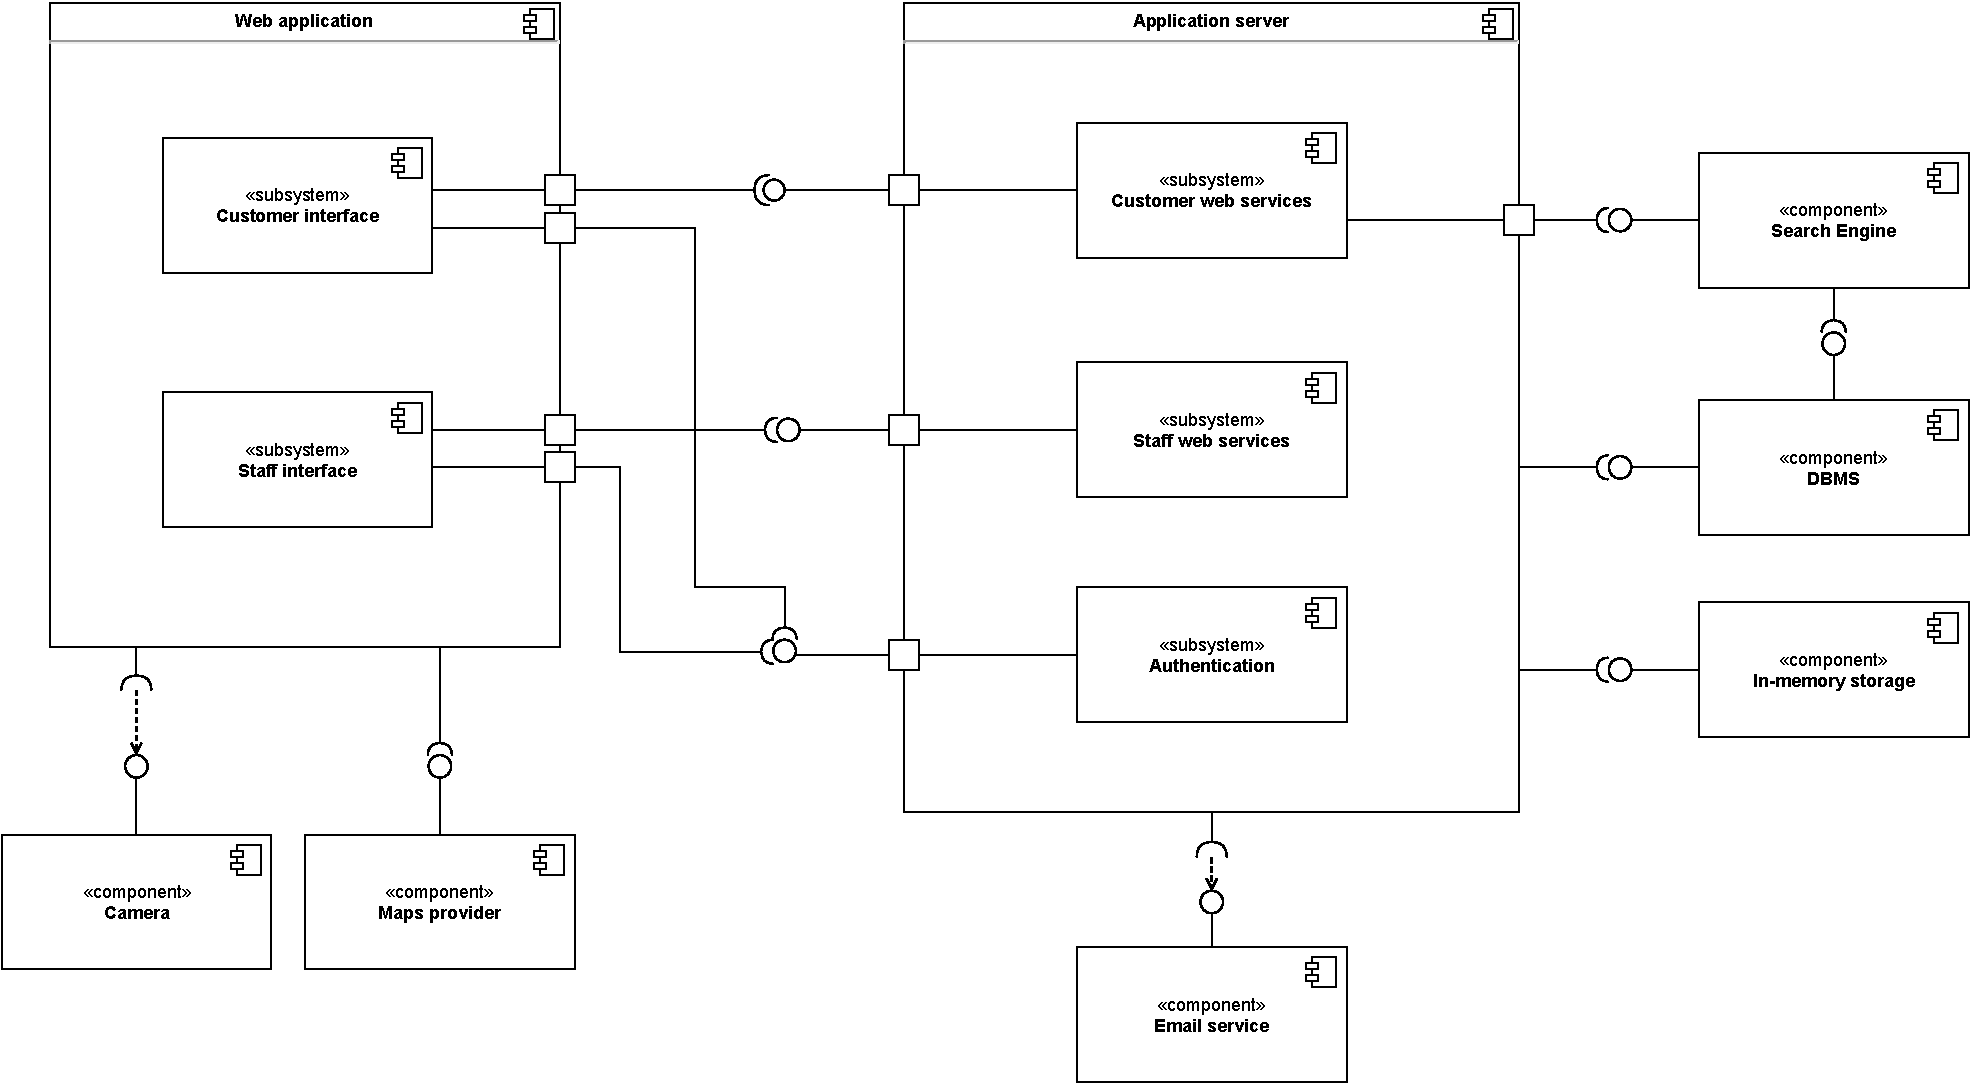
\includegraphics[width=.85\textwidth]{Images/component.pdf}
    \caption{\label{fig:component_diagram} Component diagram of the full system}
\end{figure}

In this section, an UML component diagram is used to show the internal structure of the \emph{CLup} system.
The architecture is minimal, having only a small number of internal components and a few external service providers. It is subdivided into a Web Application and an Application Server, with the respective dependencies.
In particular, the Web application needs a Camera module to scan the QR codes and an optional Maps Provider to show directions to the chosen Shop; the Application server needs a DBMS, an in-memory data store and a search engine.
The relationships and interfaces between the components are represented through assembly connectors and delegation connectors. 
A more specific description of each component follows:
\linebreak

\noindent\textbf{Web application}\\\\
\emph{CLup} is a distributed system, therefore part of the logic is included in the client. The Web Application client consists of two main components and some external interfaces:
\begin{itemize}
    \item \textbf{Customer interface}\\ The Customer can interact with a Web application that queries the Application server under the hood. The applicaition guides the user through the creation of a Ticket or a Booking displaying useful data and sending the Customer choices to the server only after validation, so that invalid input can be blocked without putting strain on the server.
    \item \textbf{Staff interface}\\ The Staff can access a special module of the interface that works in a similar way to the Customer interface, but features different functionalities. 
    
\end{itemize}
\noindent\textbf{Web application external Interfaces}
\begin{itemize}
    \item \textbf{Camera}\\ It is a requirement for the clerks to have a working camera on their device to be able to take photos of the QR codes of customers. The conversion is managed locally in the web browser and will produce an identifier that can be sent to the Application server. 
    \item \textbf{Maps provider}\\ After generating a Ticket the Users can choose to display a Map with directions to the Shop. This is possible with the help of an external Maps service provider.
\end{itemize}

\noindent\textbf{Application server}\\\\
\todo{intro}
\begin{itemize}
    \item \textbf{Customer web services}\\ It provides a REST API that is open to the Internet, which will be queried by the Web App when the user is logged in as a Customer. It makes use of the Search Engine module to provide accurate Shop results, of the In-memory storage to obtain the data relative to the current session, and of the DBMS to retrieve the persistent information that is necessary to the API.
    \item \textbf{Staff web services}\\ With a similar interface and dependencies to the above, it provides a REST API intended to be used by the Staff: store managers and clerks. \todo{More on functionalities}
    \item \textbf{Authentication}\\ This component manages the registration and login of any category of user. Given the credentials of the user by any other component, it can perform a registration or a login and generate a valid session. Its interface accepts session data to confirm a user has previously logged in and has a valid session.
    
\end{itemize}
\noindent\textbf{Application server external Interfaces}
\begin{itemize}
    \item \textbf{Search Engine}\\ This component generates real-time Shop results for every query Customers make on the homepage of the Web application.
    \item \textbf{DBMS}\\ All of the data regarding Shops, Bookings, Tickets and Customers is stored in a relational database that is managed through a DBMS, e.g. PostgreSQL. Its interface is connected to every component of the Application server.
    \item \textbf{In-memory storage}\\ Session and cache data are stored in a in-memory data store to enhance performance.
    \item \textbf{Email service}\\ It provides the capability to send emails to new Customers to validate their email address.
\end{itemize}




\subsection{Deployment view}
The distribution of device and artifacts representing the topology of the system is pictured with a deployment diagram.
The system is structured in a 2-tier architecture: the first tier is a series of Web servers, each running a reverse proxy that routes traffic to the Application servers, where the CLup binary is hosted together with a in-memory data store; the second tier is a Database server, receiving connections from the Application servers.
\begin{figure}[H]
    \centering
    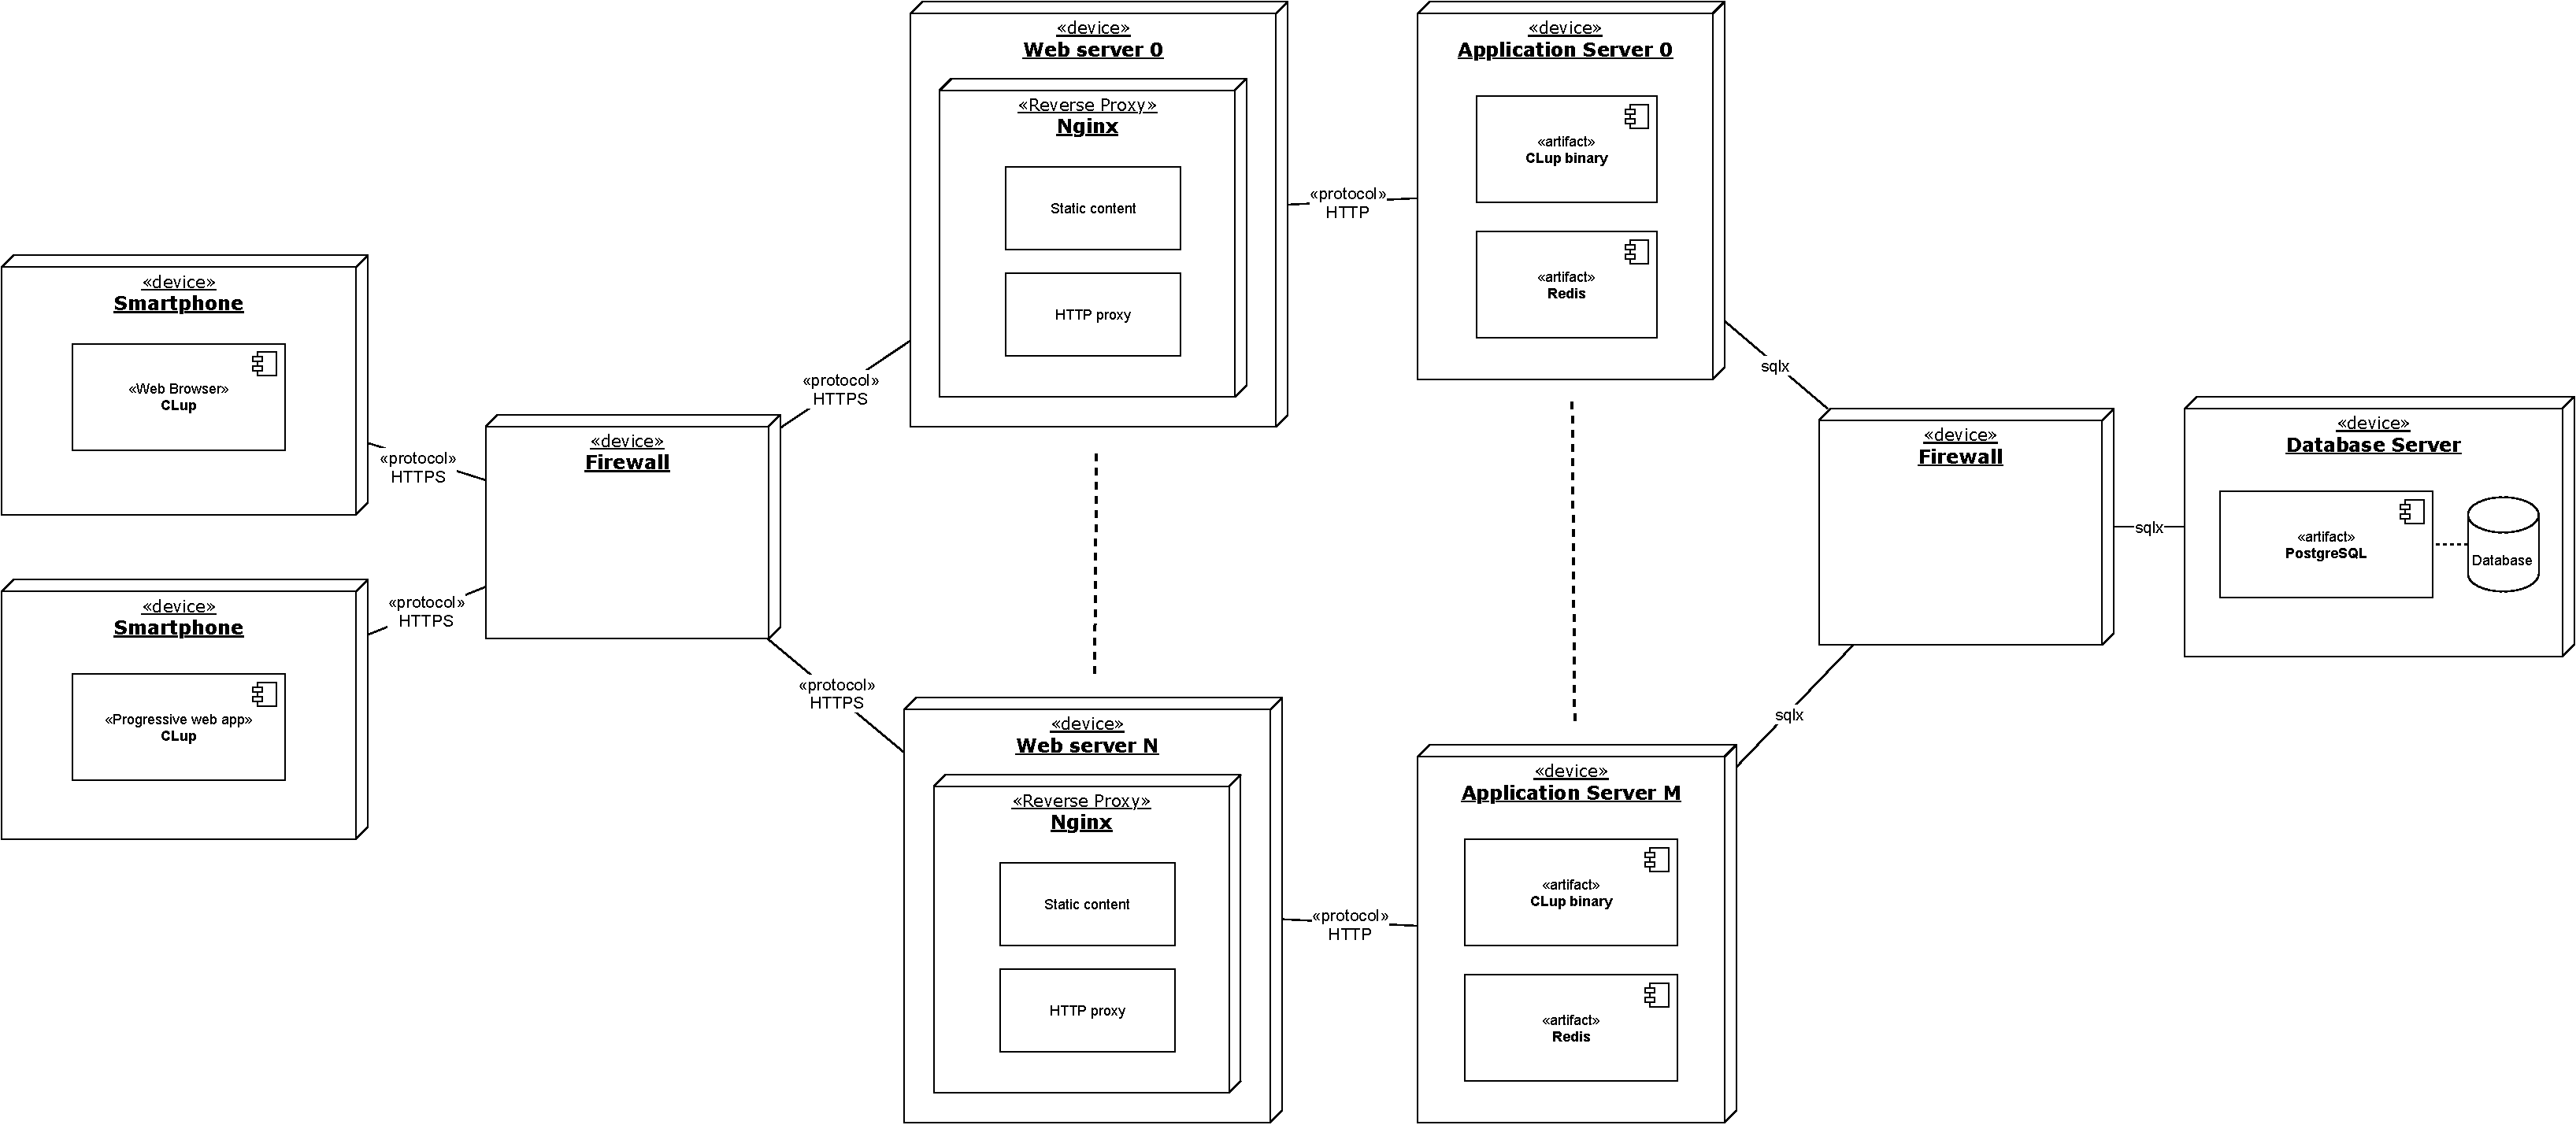
\includegraphics[width=1\textwidth]{Images/deployment-1.pdf}
    \caption{Deployment Diagram}
\end{figure}
\newpage
The same system can also be deployed with a containerized structure, as explained in the RASD. This makes setup easier, thus more portable, as it is agnostic with respect to the environment.
\begin{figure}[H]
    \centering
    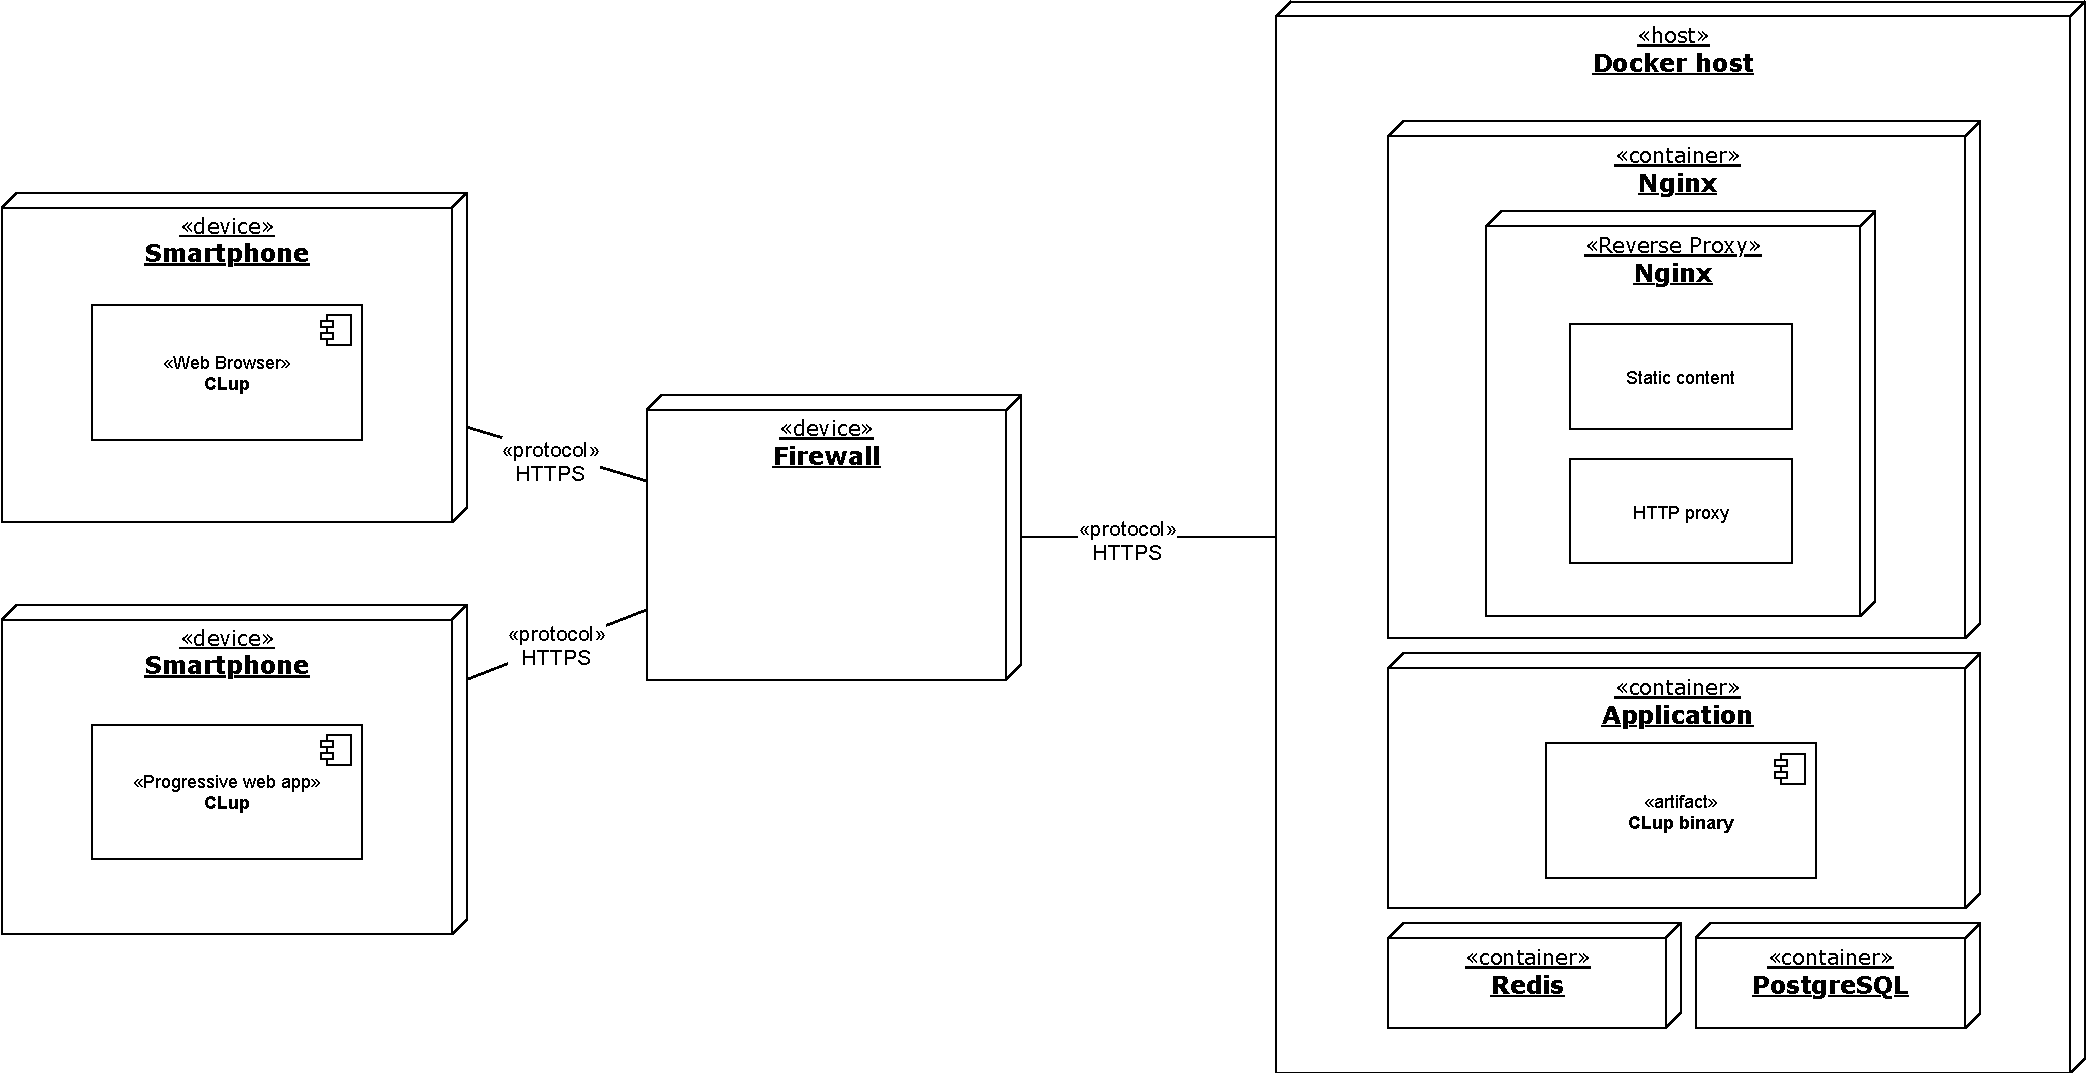
\includegraphics[width=1\textwidth]{Images/deployment-2.pdf}
    \caption{Deployment Diagram using Docker containers}
\end{figure}

\subsection{Runtime view}

\subsection{Component interfaces}

\subsection{Selected architectural styles and patterns}

\subsection{Other design decisions}
